\input format

\usepackage{tikz}
\usepackage{graphicx}
\usepackage{amssymb}
\usepackage{amsmath}
\usepackage{harpoon}
\usepackage{float}
\usepackage{enumerate}
\usepackage{algorithm}
\usepackage{algpseudocode}
\usepackage{subcaption}
\usepackage{bm}
\usepackage{listings}


\usetikzlibrary{fit,positioning}

\begin{document}
\begin{flushleft}

\bf{DD2424 Assignment 1 Report (For Basic Part)} \\
\bf{Zesen Wang} \\



\end{flushleft}



\section{Estimate Relative Error}

In the Matlab program, I set eps as ``1e-12''. And I use the formula on the manual which is
\[
	e_r=\frac{|g_a-g_n|}{\max(eps, |g_a|+|g_n|)}
\]

Then it computes the mean relative error for each entry. It uses the first 100 sets of datam and it sets $\lambda=0.1$. The program returns the result
\[
	e_W = 1.2332\cdot 10^{-7},\,\,\,\,e_b=8.2818\cdot 10^{-9}
\]

The results indicate that the implement of analytical gradient is valid.

\section{Training Results for Different Parameters}

The settings of parameters for each experiment and the accuracy on test set is shown below.

\begin{verbatim}
lambda=0, n_epochs=40, n_batch=100, eta=0.1; test_accuracy=0.1919
\end{verbatim}

\begin{figure}[h!]
	\centering
	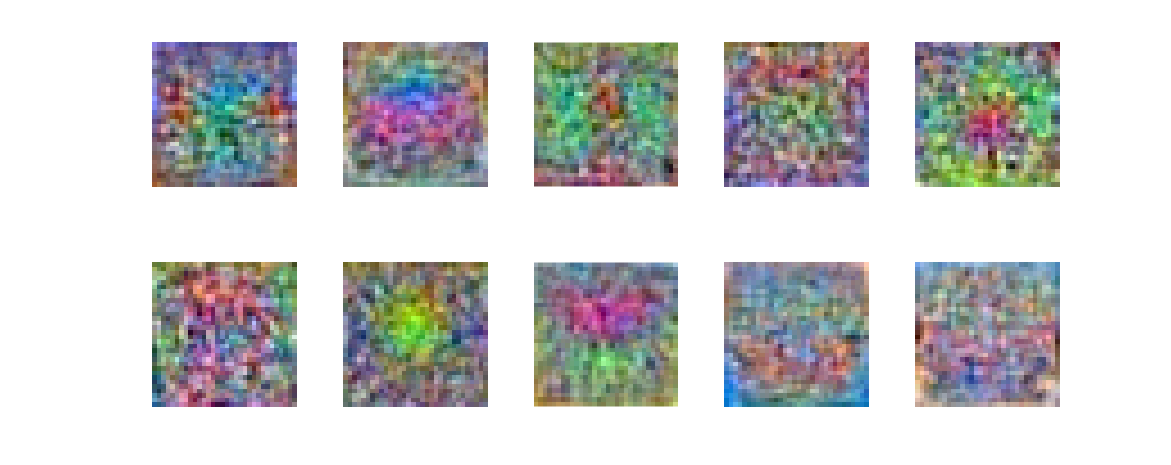
\includegraphics[width=0.65\textwidth]{../Result_Pics/w1.png}
\end{figure}

\begin{figure}[h!]
	\centering
	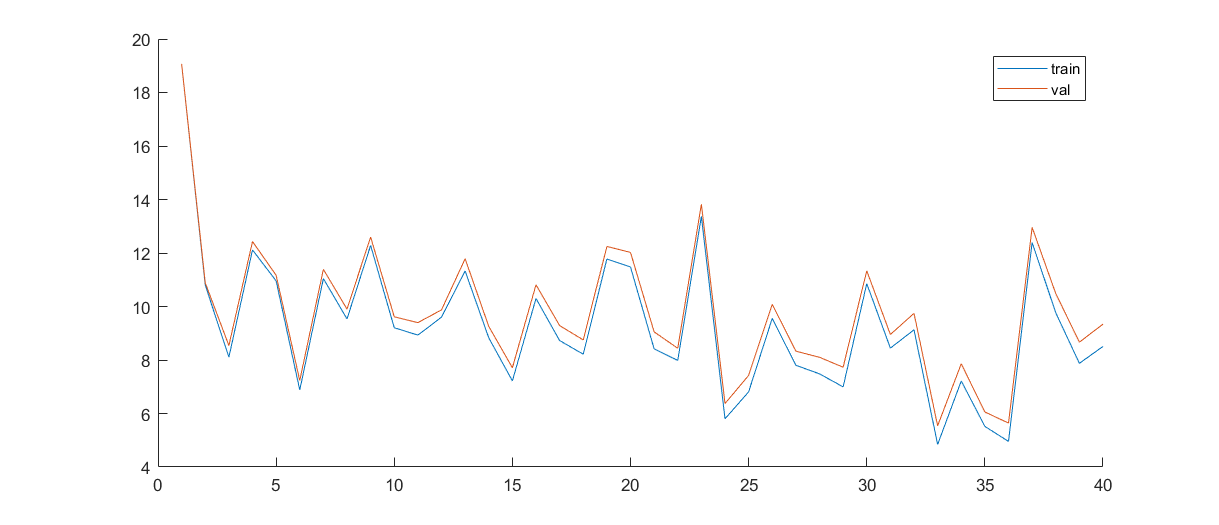
\includegraphics[width=0.65\textwidth]{../Result_Pics/a1.png}
\end{figure}

\newpage
\begin{verbatim}
lambda=0, n_epochs=40, n_batch=100, eta=0.01; test_accuracy=0.3665
\end{verbatim}

\begin{figure}[h!]
	\centering
	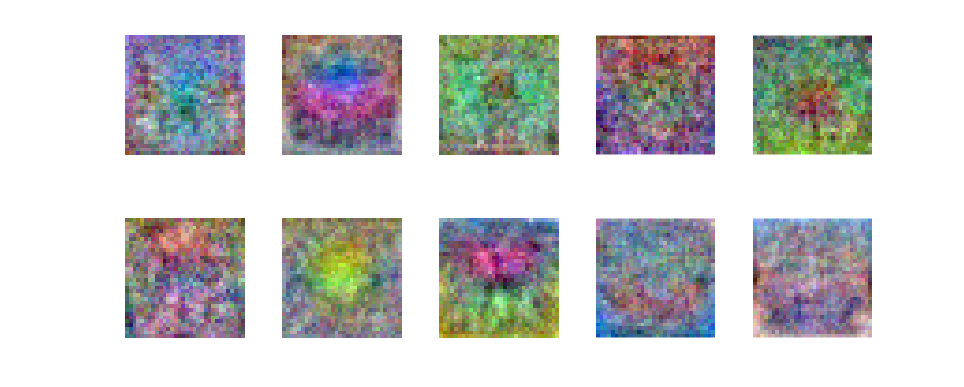
\includegraphics[width=0.65\textwidth]{../Result_Pics/w2.png}
\end{figure}

\begin{figure}[h!]
	\centering
	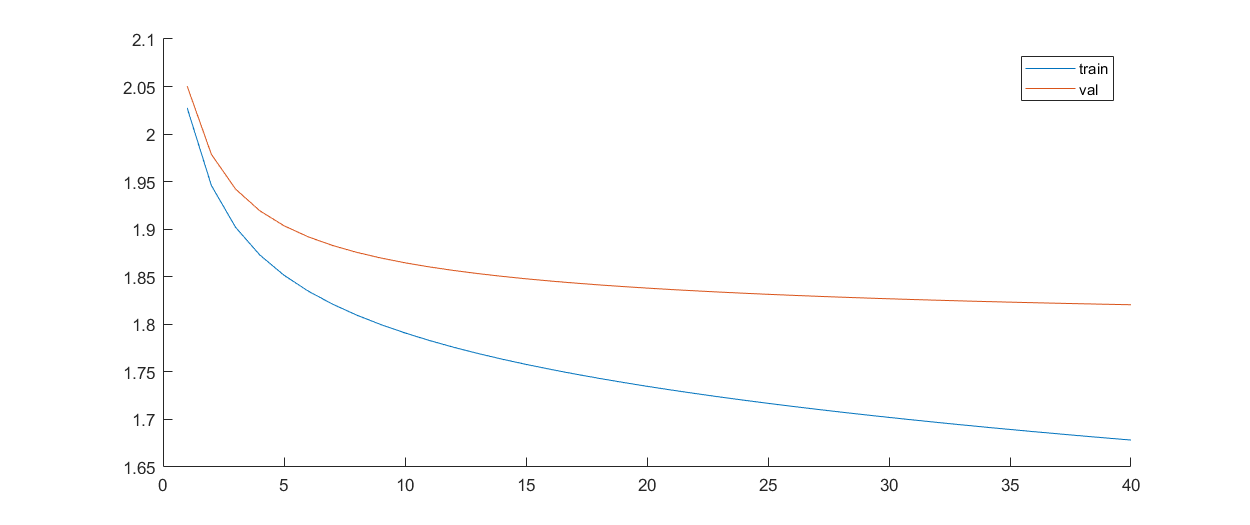
\includegraphics[width=0.65\textwidth]{../Result_Pics/a2.png}
\end{figure}

\begin{verbatim}
lambda=0.1, n_epochs=40, n_batch=100, eta=0.01; test_accuracy=0.3337
\end{verbatim}

\begin{figure}[h!]
	\centering
	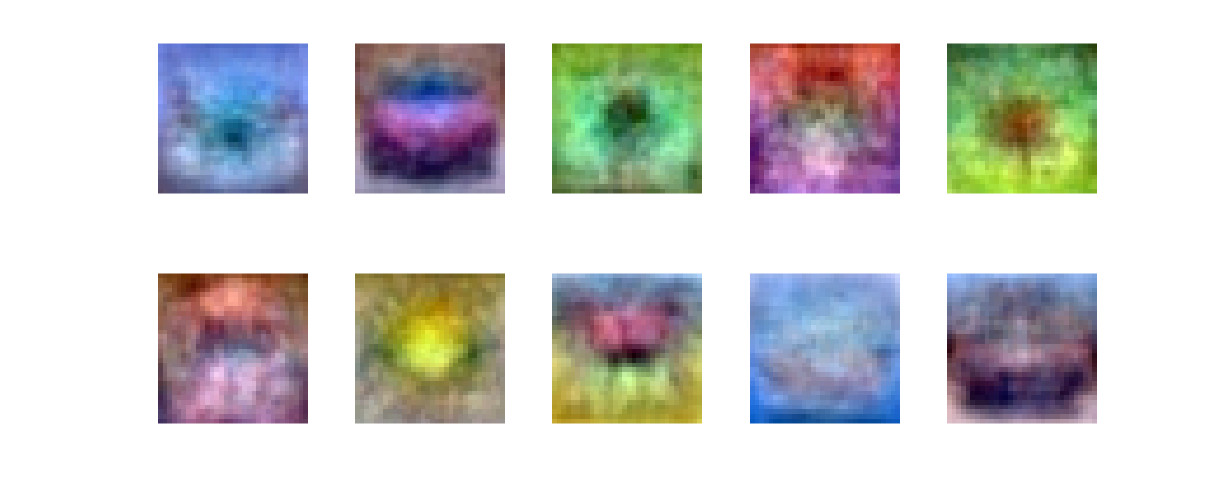
\includegraphics[width=0.65\textwidth]{../Result_Pics/w3.png}
\end{figure}

\begin{figure}[h!]
	\centering
	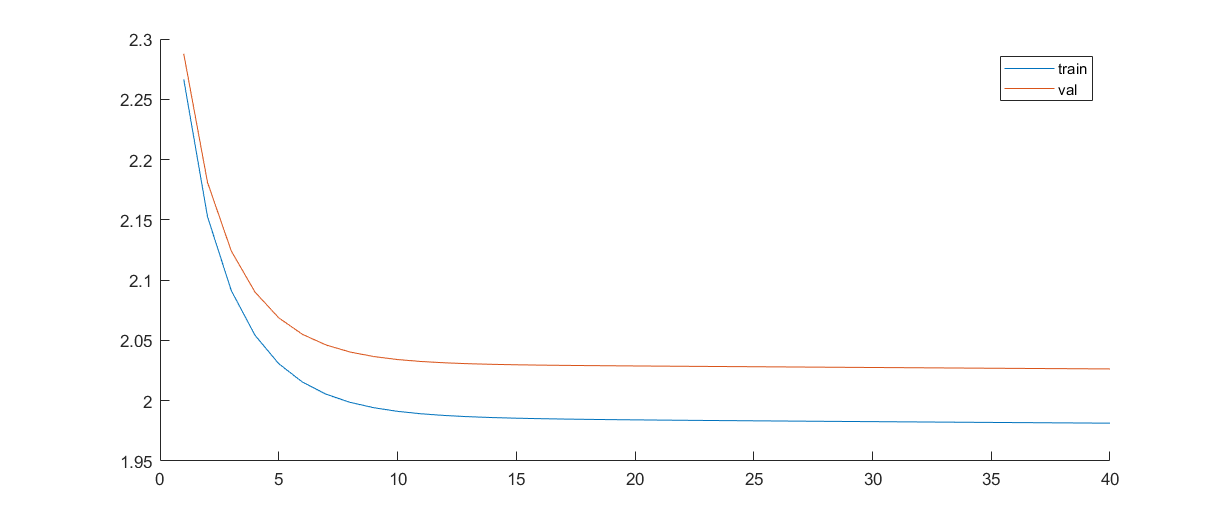
\includegraphics[width=0.65\textwidth]{../Result_Pics/a3.png}
\end{figure}

\newpage
\begin{verbatim}
lambda=1, n_epochs=40, n_batch=100, eta=0.01; test_accuracy=0.2192
\end{verbatim}

\begin{figure}[h!]
	\centering
	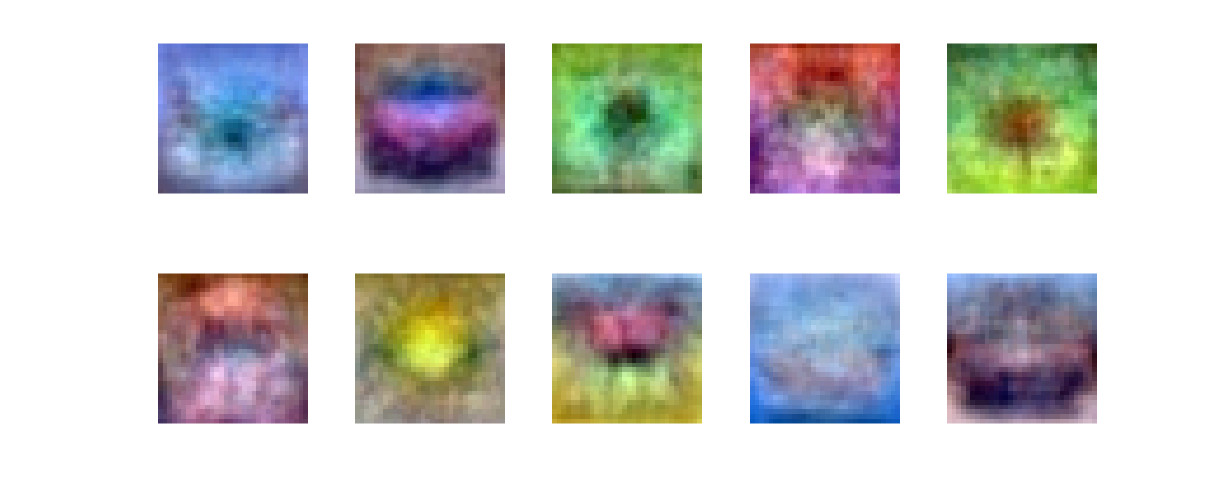
\includegraphics[width=0.65\textwidth]{../Result_Pics/w3.png}
\end{figure}

\begin{figure}[h!]
	\centering
	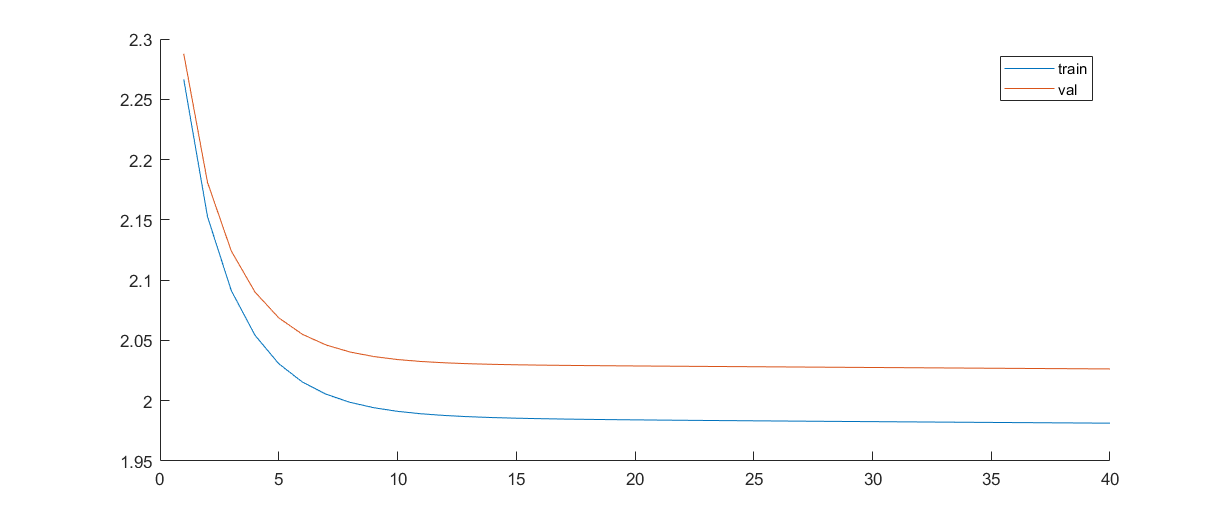
\includegraphics[width=0.65\textwidth]{../Result_Pics/a3.png}
\end{figure}

Since it's known that the underlying problem can not be solved using a one-layer network, the model is underfitting even without regularization term. Therefore, regularization term is unnecessary in this case. Increasing the amount of regularization, the network will tend to be more underfitting because the regularization term will overwhelm the data loss, which makes the loss function not reasonable. From the last three experiments, it indicates that enlarging regularization term reduces the generalization ability of model.

When the learning rate is too large (as in the first case), it makes the training unstable and hard to converge. When the learning rate is too small, it makes the training slow, which means it takes more epochs to obtain a satisfying result. Therefore, it is important to choose a correct learning rate.

\end{document}


